\documentclass{standalone}
\usepackage{tikz}
\usetikzlibrary{patterns, positioning}

\begin{document}
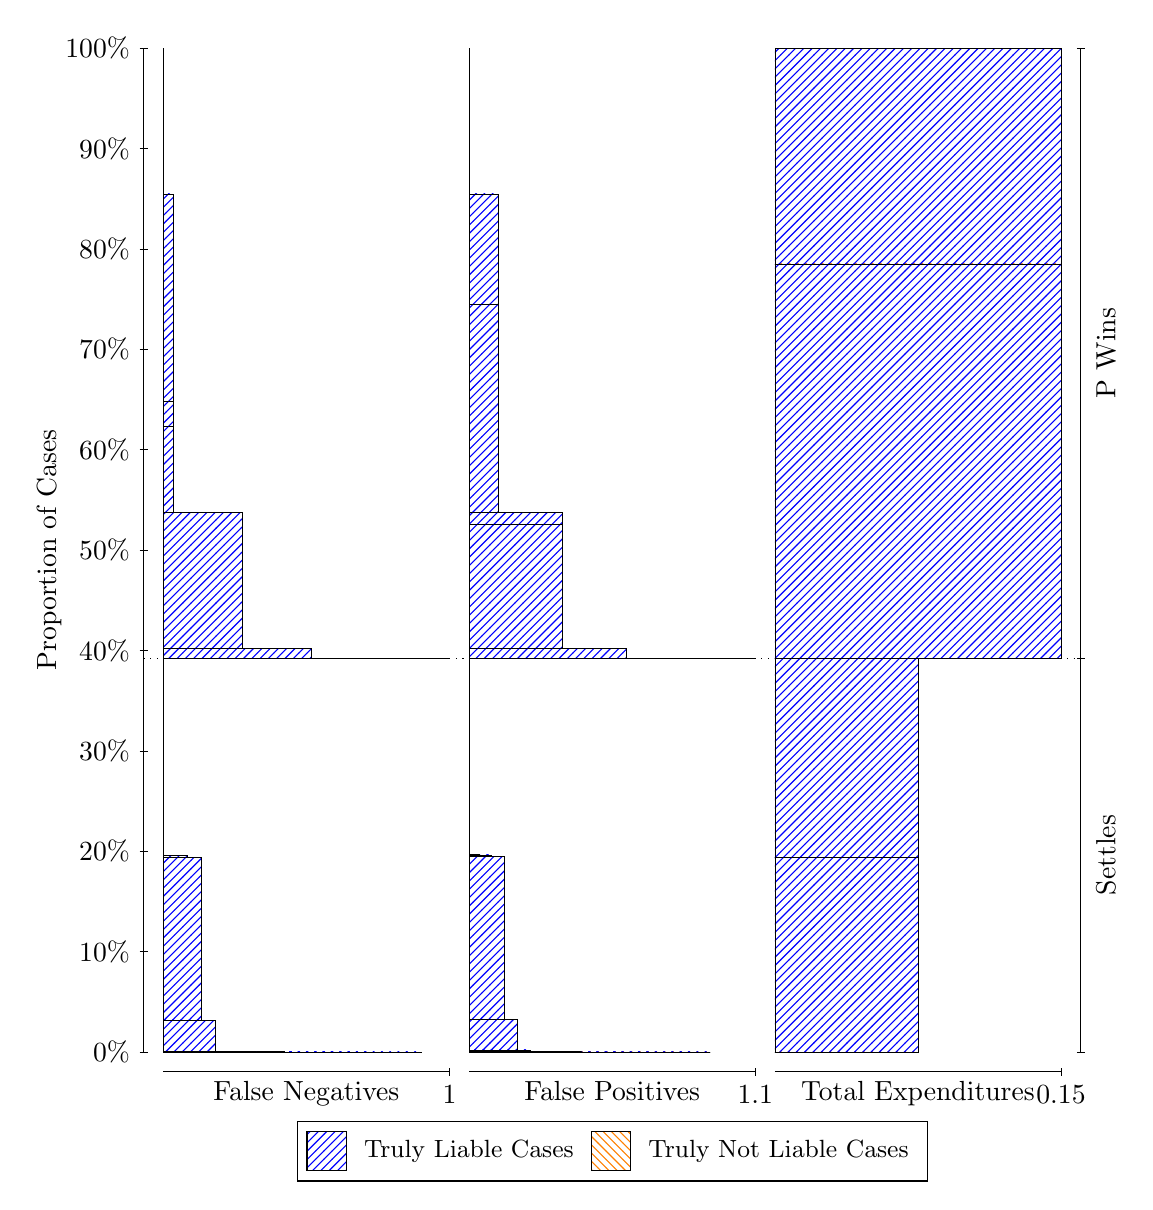
\begin{tikzpicture}
\draw[black, very thin] (1.5,1.75) -- (1.5,14.5);
\node[rotate=90, anchor=center] at (0.3, 8.125) {Proportion of Cases};
\draw[black, very thin] (1.45,1.75) -- (1.55,1.75);
\node[anchor=east] at (1.45, 1.75) {0\%};
\draw[black, very thin] (1.45,3.025) -- (1.55,3.025);
\node[anchor=east] at (1.45, 3.025) {10\%};
\draw[black, very thin] (1.45,4.3) -- (1.55,4.3);
\node[anchor=east] at (1.45, 4.3) {20\%};
\draw[black, very thin] (1.45,5.575) -- (1.55,5.575);
\node[anchor=east] at (1.45, 5.575) {30\%};
\draw[black, very thin] (1.45,6.85) -- (1.55,6.85);
\node[anchor=east] at (1.45, 6.85) {40\%};
\draw[black, very thin] (1.45,8.125) -- (1.55,8.125);
\node[anchor=east] at (1.45, 8.125) {50\%};
\draw[black, very thin] (1.45,9.4) -- (1.55,9.4);
\node[anchor=east] at (1.45, 9.4) {60\%};
\draw[black, very thin] (1.45,10.675) -- (1.55,10.675);
\node[anchor=east] at (1.45, 10.675) {70\%};
\draw[black, very thin] (1.45,11.95) -- (1.55,11.95);
\node[anchor=east] at (1.45, 11.95) {80\%};
\draw[black, very thin] (1.45,13.225) -- (1.55,13.225);
\node[anchor=east] at (1.45, 13.225) {90\%};
\draw[black, very thin] (1.45,14.5) -- (1.55,14.5);
\node[anchor=east] at (1.45, 14.5) {100\%};

\draw[black, very thin] (13.4,1.75) -- (13.4,14.5);
\draw[black, very thin] (13.35,1.75) -- (13.45,1.75);
\node[anchor=west] at (13.35, 1.75) {};
\draw[black, very thin] (13.35,6.752) -- (13.45,6.752);
\node[anchor=west] at (13.35, 6.752) {};
\draw[black, very thin] (13.35,14.5) -- (13.45,14.5);
\node[anchor=west] at (13.35, 14.5) {};

\draw[black, very thin, pattern color=blue, pattern=north east lines] (1.75,1.75) rectangle (5.0331,1.75);
\draw[black, very thin, pattern color=blue, pattern=north east lines] (1.75,1.75) rectangle (4.3327,1.75);
\draw[black, very thin, pattern color=blue, pattern=north east lines] (1.75,1.75) rectangle (4.1576,1.75);
\draw[black, very thin, pattern color=blue, pattern=north east lines] (1.75,1.75) rectangle (3.9825,1.75);
\draw[black, very thin, pattern color=blue, pattern=north east lines] (1.75,1.75) rectangle (3.6323,1.75);
\draw[black, very thin, pattern color=blue, pattern=north east lines] (1.75,1.75) rectangle (3.4572,1.75);
\draw[black, very thin, pattern color=blue, pattern=north east lines] (1.75,1.75) rectangle (3.2821,1.7532);
\draw[black, very thin, pattern color=blue, pattern=north east lines] (1.75,1.7532) rectangle (3.107,1.7532);
\draw[black, very thin, pattern color=blue, pattern=north east lines] (1.75,1.7532) rectangle (2.9319,1.7532);
\draw[black, very thin, pattern color=blue, pattern=north east lines] (1.75,1.7532) rectangle (2.7568,1.7534);
\draw[black, very thin, pattern color=blue, pattern=north east lines] (1.75,1.7534) rectangle (2.5817,1.7535);
\draw[black, very thin, pattern color=blue, pattern=north east lines] (1.75,1.7535) rectangle (2.5817,1.7545);
\draw[black, very thin, pattern color=blue, pattern=north east lines] (1.75,1.7545) rectangle (2.4066,2.1561);
\draw[black, very thin, pattern color=blue, pattern=north east lines] (1.75,2.1561) rectangle (2.2315,2.1562);
\draw[black, very thin, pattern color=blue, pattern=north east lines] (1.75,2.1562) rectangle (2.2315,4.2243);
\draw[black, very thin, pattern color=blue, pattern=north east lines] (1.75,4.2243) rectangle (2.0564,4.2441);
\draw[black, very thin, pattern color=blue, pattern=north east lines] (1.75,4.2441) rectangle (1.8813,4.249);
\draw[black, very thin, pattern color=orange, pattern=north west lines] (1.75,4.249) rectangle (1.75,4.249);
\draw[black, very thin, pattern color=blue, pattern=north east lines] (1.75,4.249) rectangle (1.75,6.752);
\draw[black, very thin, pattern color=blue, pattern=north east lines] (1.75,6.752) rectangle (5.3833,6.752);
\draw[black, very thin, pattern color=blue, pattern=north east lines] (1.75,6.752) rectangle (4.5078,6.7532);
\draw[black, very thin, pattern color=blue, pattern=north east lines] (1.75,6.7532) rectangle (3.6323,6.8722);
\draw[black, very thin, pattern color=blue, pattern=north east lines] (1.75,6.8722) rectangle (2.7568,8.6025);
\draw[black, very thin, pattern color=blue, pattern=north east lines] (1.75,8.6025) rectangle (1.8813,9.6904);
\draw[black, very thin, pattern color=blue, pattern=north east lines] (1.75,9.6904) rectangle (1.8813,10.009);
\draw[black, very thin, pattern color=blue, pattern=north east lines] (1.75,10.009) rectangle (1.8813,12.649);
\draw[black, very thin, pattern color=orange, pattern=north west lines] (1.75,12.649) rectangle (1.75,12.649);
\draw[black, very thin, pattern color=blue, pattern=north east lines] (1.75,12.649) rectangle (1.75,14.5);
\draw[black, very thin, pattern color=orange, pattern=north west lines] (5.6333,1.75) rectangle (8.6951,1.75);
\draw[black, very thin, pattern color=blue, pattern=north east lines] (5.6333,1.75) rectangle (8.6951,1.75);
\draw[black, very thin, pattern color=orange, pattern=north west lines] (5.6333,1.75) rectangle (8.3685,1.75);
\draw[black, very thin, pattern color=blue, pattern=north east lines] (5.6333,1.75) rectangle (8.3685,1.75);
\draw[black, very thin, pattern color=orange, pattern=north west lines] (5.6333,1.75) rectangle (8.0419,1.75);
\draw[black, very thin, pattern color=blue, pattern=north east lines] (5.6333,1.75) rectangle (8.0419,1.75);
\draw[black, very thin, pattern color=blue, pattern=north east lines] (5.6333,1.75) rectangle (7.8787,1.75);
\draw[black, very thin, pattern color=orange, pattern=north west lines] (5.6333,1.75) rectangle (7.7154,1.75);
\draw[black, very thin, pattern color=blue, pattern=north east lines] (5.6333,1.75) rectangle (7.7154,1.75);
\draw[black, very thin, pattern color=blue, pattern=north east lines] (5.6333,1.75) rectangle (7.5521,1.75);
\draw[black, very thin, pattern color=orange, pattern=north west lines] (5.6333,1.75) rectangle (7.3888,1.75);
\draw[black, very thin, pattern color=blue, pattern=north east lines] (5.6333,1.75) rectangle (7.3888,1.75);
\draw[black, very thin, pattern color=blue, pattern=north east lines] (5.6333,1.75) rectangle (7.2255,1.7502);
\draw[black, very thin, pattern color=blue, pattern=north east lines] (5.6333,1.7502) rectangle (7.0622,1.7526);
\draw[black, very thin, pattern color=orange, pattern=north west lines] (5.6333,1.7526) rectangle (7.0622,1.7526);
\draw[black, very thin, pattern color=blue, pattern=north east lines] (5.6333,1.7526) rectangle (7.0622,1.7526);
\draw[black, very thin, pattern color=blue, pattern=north east lines] (5.6333,1.7526) rectangle (6.8989,1.7528);
\draw[black, very thin, pattern color=blue, pattern=north east lines] (5.6333,1.7528) rectangle (6.7356,1.7536);
\draw[black, very thin, pattern color=orange, pattern=north west lines] (5.6333,1.7536) rectangle (6.7356,1.7536);
\draw[black, very thin, pattern color=blue, pattern=north east lines] (5.6333,1.7536) rectangle (6.7356,1.7536);
\draw[black, very thin, pattern color=blue, pattern=north east lines] (5.6333,1.7536) rectangle (6.5723,1.7538);
\draw[black, very thin, pattern color=blue, pattern=north east lines] (5.6333,1.7538) rectangle (6.409,1.7774);
\draw[black, very thin, pattern color=blue, pattern=north east lines] (5.6333,1.7774) rectangle (6.2457,2.1601);
\draw[black, very thin, pattern color=blue, pattern=north east lines] (5.6333,2.1601) rectangle (6.2457,2.1603);
\draw[black, very thin, pattern color=orange, pattern=north west lines] (5.6333,2.1603) rectangle (6.0824,2.1603);
\draw[black, very thin, pattern color=blue, pattern=north east lines] (5.6333,2.1603) rectangle (6.0824,4.2294);
\draw[black, very thin, pattern color=blue, pattern=north east lines] (5.6333,4.2294) rectangle (6.0824,4.2341);
\draw[black, very thin, pattern color=blue, pattern=north east lines] (5.6333,4.2341) rectangle (5.9191,4.2528);
\draw[black, very thin, pattern color=blue, pattern=north east lines] (5.6333,4.2528) rectangle (5.9191,4.2529);
\draw[black, very thin, pattern color=blue, pattern=north east lines] (5.6333,4.2529) rectangle (5.7558,4.2579);
\draw[black, very thin, pattern color=blue, pattern=north east lines] (5.6333,4.2579) rectangle (5.6333,6.752);
\draw[black, very thin, pattern color=orange, pattern=north west lines] (5.6333,6.752) rectangle (9.2667,6.752);
\draw[black, very thin, pattern color=blue, pattern=north east lines] (5.6333,6.752) rectangle (9.2667,6.752);
\draw[black, very thin, pattern color=orange, pattern=north west lines] (5.6333,6.752) rectangle (8.4502,6.752);
\draw[black, very thin, pattern color=blue, pattern=north east lines] (5.6333,6.752) rectangle (8.4502,6.7532);
\draw[black, very thin, pattern color=orange, pattern=north west lines] (5.6333,6.7532) rectangle (7.6337,6.7532);
\draw[black, very thin, pattern color=blue, pattern=north east lines] (5.6333,6.7532) rectangle (7.6337,6.8727);
\draw[black, very thin, pattern color=blue, pattern=north east lines] (5.6333,6.8727) rectangle (6.8172,8.4552);
\draw[black, very thin, pattern color=orange, pattern=north west lines] (5.6333,8.4552) rectangle (6.8172,8.4552);
\draw[black, very thin, pattern color=blue, pattern=north east lines] (5.6333,8.4552) rectangle (6.8172,8.6029);
\draw[black, very thin, pattern color=blue, pattern=north east lines] (5.6333,8.6029) rectangle (6.0007,11.243);
\draw[black, very thin, pattern color=orange, pattern=north west lines] (5.6333,11.243) rectangle (6.0007,11.243);
\draw[black, very thin, pattern color=blue, pattern=north east lines] (5.6333,11.243) rectangle (6.0007,12.649);
\draw[black, very thin, pattern color=blue, pattern=north east lines] (5.6333,12.649) rectangle (5.6333,14.5);
\draw[black, very thin, pattern color=orange, pattern=north west lines] (9.5167,1.75) rectangle (11.333,1.75);
\draw[black, very thin, pattern color=blue, pattern=north east lines] (9.5167,1.75) rectangle (11.333,4.2237);
\draw[black, very thin, pattern color=orange, pattern=north west lines] (9.5167,4.2237) rectangle (11.333,4.2237);
\draw[black, very thin, pattern color=blue, pattern=north east lines] (9.5167,4.2237) rectangle (11.333,6.752);
\draw[black, very thin, pattern color=orange, pattern=north west lines] (9.5167,6.752) rectangle (13.15,6.752);
\draw[black, very thin, pattern color=blue, pattern=north east lines] (9.5167,6.752) rectangle (13.15,11.758);
\draw[black, very thin, pattern color=orange, pattern=north west lines] (9.5167,11.758) rectangle (13.15,11.758);
\draw[black, very thin, pattern color=blue, pattern=north east lines] (9.5167,11.758) rectangle (13.15,14.5);
\draw[black, dotted] (1.5,6.752) -- (13.4,6.752);
\draw[black, very thin] (1.75,1.5) -- (5.3833,1.5);
\node[anchor=north] at (3.5667, 1.5) {False Negatives};
\draw[black, very thin] (5.3833,1.45) -- (5.3833,1.55);
\node[anchor=north] at (5.3833, 1.45) {1};

\draw[black, very thin] (5.6333,1.5) -- (9.2667,1.5);
\node[anchor=north] at (7.45, 1.5) {False Positives};
\draw[black, very thin] (9.2667,1.45) -- (9.2667,1.55);
\node[anchor=north] at (9.2667, 1.45) {1.1};

\draw[black, very thin] (9.5167,1.5) -- (13.15,1.5);
\node[anchor=north] at (11.333, 1.5) {Total Expenditures};
\draw[black, very thin] (13.15,1.45) -- (13.15,1.55);
\node[anchor=north] at (13.15, 1.45) {0.15};

\node[black, centered, rotate=90] at (13.72, 4.251) {Settles};
\node[black, centered, rotate=90] at (13.72, 10.626) {P Wins};

\draw (7.449999999999999,1.5) node[draw=none] (baseCoordinate) {};
\begin{scope}[align=center]
        \matrix[scale=0.5, draw=black, below=0.5cm of baseCoordinate, nodes={draw}, column sep=0.1cm]{
            \node[rectangle, draw, minimum width=0.5cm, minimum height=0.5cm, pattern=north east lines, pattern color=blue] {}; &
            \node[draw=none, font=\small] (B) {Truly Liable Cases}; &
            \node[rectangle, draw, minimum width=0.5cm, minimum height=0.5cm, pattern=north west lines, pattern color=orange] {}; &
            \node[draw=none, font=\small] (B) {Truly Not Liable Cases}; \\
            };
\end{scope}

\end{tikzpicture}
\end{document}